\documentclass[10pt,]{article}
\usepackage{lmodern}
\usepackage{amssymb,amsmath}
\usepackage{ifxetex,ifluatex}
\usepackage{fixltx2e} % provides \textsubscript
\ifnum 0\ifxetex 1\fi\ifluatex 1\fi=0 % if pdftex
  \usepackage[T1]{fontenc}
  \usepackage[utf8]{inputenc}
\else % if luatex or xelatex
  \ifxetex
    \usepackage{mathspec}
    \usepackage{xltxtra,xunicode}
  \else
    \usepackage{fontspec}
  \fi
  \defaultfontfeatures{Mapping=tex-text,Scale=MatchLowercase}
  \newcommand{\euro}{€}
\fi
% use upquote if available, for straight quotes in verbatim environments
\IfFileExists{upquote.sty}{\usepackage{upquote}}{}
% use microtype if available
\IfFileExists{microtype.sty}{%
\usepackage{microtype}
\UseMicrotypeSet[protrusion]{basicmath} % disable protrusion for tt fonts
}{}
\usepackage[margin=0.5in]{geometry}
\usepackage{longtable,booktabs}
\usepackage{graphicx}
\makeatletter
\def\maxwidth{\ifdim\Gin@nat@width>\linewidth\linewidth\else\Gin@nat@width\fi}
\def\maxheight{\ifdim\Gin@nat@height>\textheight\textheight\else\Gin@nat@height\fi}
\makeatother
% Scale images if necessary, so that they will not overflow the page
% margins by default, and it is still possible to overwrite the defaults
% using explicit options in \includegraphics[width, height, ...]{}
\setkeys{Gin}{width=\maxwidth,height=\maxheight,keepaspectratio}
\ifxetex
  \usepackage[setpagesize=false, % page size defined by xetex
              unicode=false, % unicode breaks when used with xetex
              xetex]{hyperref}
\else
  \usepackage[unicode=true]{hyperref}
\fi
\hypersetup{breaklinks=true,
            bookmarks=true,
            pdfauthor={PMG Group},
            pdftitle={QA0 Report},
            colorlinks=true,
            citecolor=blue,
            urlcolor=blue,
            linkcolor=magenta,
            pdfborder={0 0 0}}
\urlstyle{same}  % don't use monospace font for urls
\setlength{\parindent}{0pt}
\setlength{\parskip}{6pt plus 2pt minus 1pt}
\setlength{\emergencystretch}{3em}  % prevent overfull lines
\setcounter{secnumdepth}{5}

%%% Use protect on footnotes to avoid problems with footnotes in titles
\let\rmarkdownfootnote\footnote%
\def\footnote{\protect\rmarkdownfootnote}

%%% Change title format to be more compact
\usepackage{titling}
\setlength{\droptitle}{-2em}
  \title{QA0 Report}
  \pretitle{\vspace{\droptitle}\centering\huge}
  \posttitle{\par}
  \author{PMG Group}
  \preauthor{\centering\large\emph}
  \postauthor{\par}
  \date{}
  \predate{}\postdate{}




\begin{document}

\maketitle


\section{EB, SB and Array
Information}\label{eb-sb-and-array-information}

\begin{longtable}[c]{@{}lr@{}}
\caption{Execution Block Information.}\tabularnewline
\toprule
& Value\tabularnewline
\midrule
\endfirsthead
\toprule
& Value\tabularnewline
\midrule
\endhead
EB UID: & uid://A002/Xa2300a/Xa8a\tabularnewline
Start Time: & 2015-06-04 02:05:01.030000\tabularnewline
Number of Scans: & 14\tabularnewline
EB Status: & SUCCESS\tabularnewline
SB UID: & uid://A002/X6b0cc1/X49\tabularnewline
SB Name: & Arp220\_B6\_low\_5\tabularnewline
Project Code: & 2012.1.00453.S\tabularnewline
Array Name: & Array004\tabularnewline
Array Family: & 12 {[}m{]}\tabularnewline
Correlator: & BL\tabularnewline
\bottomrule
\end{longtable}

\begin{longtable}[c]{@{}lr@{}}
\caption{Scheduling Block Information.}\tabularnewline
\toprule
& Value\tabularnewline
\midrule
\endfirsthead
\toprule
& Value\tabularnewline
\midrule
\endhead
SB UID: & uid://A002/X6b0cc1/X49\tabularnewline
SB Name: & Arp220\_B6\_low\_5\tabularnewline
Project Code: & 2012.1.00453.S\tabularnewline
Band: & ALMA\_RB\_06\tabularnewline
Representtive Freq.: & 218.51 GHz.\tabularnewline
RA: & 15:34:57.29\tabularnewline
DEC: & 23:30:10.48\tabularnewline
Min. Array AR (100GHz): & 0.43 arcsec.\tabularnewline
Max. Array AR (100GHz): & 1.01 arcsec.\tabularnewline
SB req. AR (100GHz): & 0.92 arcsec.\tabularnewline
SB req. LAS (100GHz): & 5.50 arcsec.\tabularnewline
Best Configuration: & C34-5\tabularnewline
\bottomrule
\end{longtable}

Num Antennas: 38.

Total Execution Time: 27.6 mins.

EB Integration Time on Source: 2.52 mins.

SB Requested Time on Source: 2.28 mins.

Is Polarization? False.

\pagebreak

\section{QA0 Summary}\label{qa0-summary}

\subsection{Check Flagged Data}\label{check-flagged-data}

No antennas with more than 10\% of data flagged.

\subsection{Check Calibration Intents}\label{check-calibration-intents}

1 scans with intent OBSERVE\_TARGET found.\newline 
1 scans with intent CALIBRATE\_BANDPASS found.\newline 
1 scans with intent CALIBRATE\_SIDEBAND\_RATIO found.\newline 
3 scans with intent CALIBRATE\_POINTING found.\newline 
1 scans with intent CALIBRATE\_AMPLI found.\newline 
2 scans with intent CALIBRATE\_PHASE found.\newline 
Pass

\subsection{Check Amplitude Cal}\label{check-amplitude-cal}

A Solar System object was used. All OK.Pass

\subsection{Check Mosaic Coverage /
Pointings}\label{check-mosaic-coverage-pointings}

Recomendation: \newline 
Pass

\subsection{Check Array Resolution}\label{check-array-resolution}

\subsection{Check Atmosphere
Calibrations}\label{check-atmosphere-calibrations}

Antenna(s) DA43 DV15 have SBgain outside spec (see details).

\subsection{Check Phase Calibrations.}\label{check-phase-calibrations.}

\subsection{Check Pointing
Calibrations.}\label{check-pointing-calibrations.}

\begin{longtable}[c]{@{}lrr@{}}
\toprule
ANTENNA & rms & limit\tabularnewline
\midrule
\endhead
DA60 & 2.694829 & 2.55678\tabularnewline
DV18 & 6.860147 & 2.55678\tabularnewline
\bottomrule
\end{longtable}

\begin{longtable}[c]{@{}lrr@{}}
\toprule
ANTENNA & rms & points\tabularnewline
\midrule
\endhead
DA60 & 2.516590 & 15\tabularnewline
DV13 & 3.927395 & 15\tabularnewline
DV16 & 4.110723 & 15\tabularnewline
DV18 & 4.855803 & 15\tabularnewline
DV20 & 3.776593 & 15\tabularnewline
\bottomrule
\end{longtable}

\subsection{Check Latest Focus.}\label{check-latest-focus.}

\subsection{Check Latest Delay.}\label{check-latest-delay.}

\pagebreak

\section{Pointing / Mosaic Details}\label{pointing-mosaic-details}

\begin{figure}[htbp]
\centering
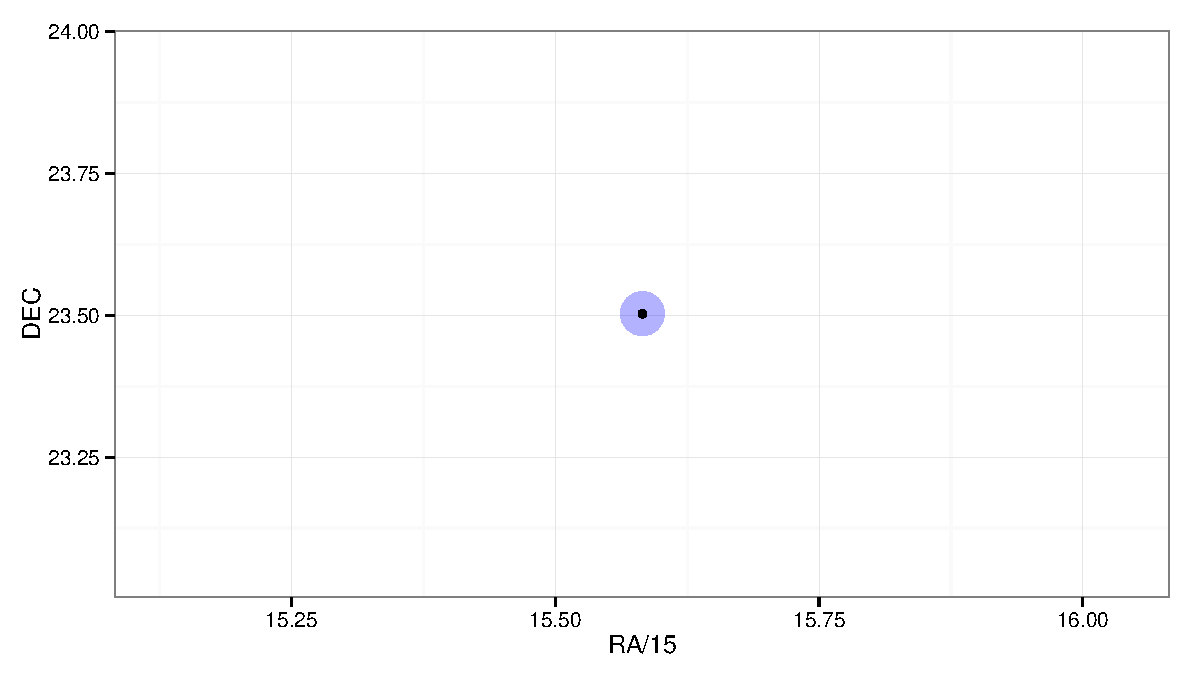
\includegraphics{QA0rep_files/figure-latex/unnamed-chunk-6-1.pdf}
\caption{}
\end{figure}

\pagebreak

\section{Scans Information}\label{scans-information}

\begin{longtable}[c]{@{}rrllll@{}}
\toprule
Scan & SubSc. & Start & End & Intent & Field\tabularnewline
\midrule
\endhead
1 & 10 & 2015-06-04 02:05:01 & 2015-06-04 02:07:21 & CALIBRATE\_POINTING
& J1550+0527\tabularnewline
2 & 2 & 2015-06-04 02:08:17 & 2015-06-04 02:09:43 &
CALIBRATE\_SIDEBAND\_RATIO & J1550+0527\tabularnewline
3 & 3 & 2015-06-04 02:09:43 & 2015-06-04 02:10:02 &
CALIBRATE\_ATMOSPHERE & J1550+0527\tabularnewline
4 & 10 & 2015-06-04 02:10:02 & 2015-06-04 02:15:43 & CALIBRATE\_BANDPASS
& J1550+0527\tabularnewline
5 & 10 & 2015-06-04 02:16:03 & 2015-06-04 02:18:21 & CALIBRATE\_POINTING
& J1517-2422\tabularnewline
6 & 3 & 2015-06-04 02:18:42 & 2015-06-04 02:19:25 &
CALIBRATE\_ATMOSPHERE & Titan\tabularnewline
7 & 5 & 2015-06-04 02:19:25 & 2015-06-04 02:22:23 & CALIBRATE\_AMPLI &
Titan\tabularnewline
8 & 10 & 2015-06-04 02:22:43 & 2015-06-04 02:25:01 & CALIBRATE\_POINTING
& J1516+1932\tabularnewline
9 & 1 & 2015-06-04 02:25:15 & 2015-06-04 02:26:15 & CALIBRATE\_PHASE &
J1516+1932\tabularnewline
10 & 3 & 2015-06-04 02:26:26 & 2015-06-04 02:27:07 &
CALIBRATE\_ATMOSPHERE & J1550+0527\tabularnewline
11 & 1 & 2015-06-04 02:27:07 & 2015-06-04 02:27:57 & CALIBRATE\_DELAY &
J1550+0527\tabularnewline
12 & 3 & 2015-06-04 02:28:09 & 2015-06-04 02:28:55 &
CALIBRATE\_ATMOSPHERE & Arp220\tabularnewline
13 & 5 & 2015-06-04 02:28:55 & 2015-06-04 02:31:47 & OBSERVE\_TARGET &
Arp220\tabularnewline
14 & 1 & 2015-06-04 02:31:53 & 2015-06-04 02:32:35 & CALIBRATE\_PHASE &
J1516+1932\tabularnewline
\bottomrule
\end{longtable}

\pagebreak

\section{Atmosphere Details}\label{atmosphere-details}

\begin{longtable}[c]{@{}rlrrrr@{}}
\toprule
SCAN & BB & trecX & trecY & tsysX & tsysY\tabularnewline
\midrule
\endhead
3 & BB\_1 & 42.59168 & 45.13751 & 79.98778 & 82.60945\tabularnewline
3 & BB\_2 & 38.71401 & 40.74519 & 74.51009 & 75.60708\tabularnewline
3 & BB\_3 & 34.05957 & 34.01127 & 75.72794 & 75.73999\tabularnewline
3 & BB\_4 & 39.31945 & 40.37367 & 83.78958 & 86.25096\tabularnewline
6 & BB\_1 & 42.32688 & 42.91869 & 77.14703 & 79.69205\tabularnewline
6 & BB\_2 & 37.81037 & 39.05960 & 72.10497 & 73.11743\tabularnewline
6 & BB\_3 & 33.53483 & 34.74098 & 72.53561 & 72.37147\tabularnewline
6 & BB\_4 & 38.79378 & 39.29923 & 79.79565 & 82.35462\tabularnewline
10 & BB\_1 & 41.08031 & 44.12023 & 79.84879 & 82.20602\tabularnewline
10 & BB\_2 & 38.27000 & 39.23594 & 74.51165 & 75.65597\tabularnewline
10 & BB\_3 & 33.41242 & 32.41963 & 75.62054 & 75.53324\tabularnewline
10 & BB\_4 & 37.82838 & 39.01030 & 83.10505 & 85.44464\tabularnewline
12 & BB\_1 & 43.08506 & 43.63559 & 86.79262 & 89.31620\tabularnewline
12 & BB\_2 & 38.15220 & 39.47245 & 81.10900 & 82.30431\tabularnewline
12 & BB\_3 & 33.90549 & 34.25163 & 83.64722 & 83.76488\tabularnewline
12 & BB\_4 & 39.07481 & 39.28326 & 92.24089 & 94.10559\tabularnewline
\bottomrule
\end{longtable}

\begin{longtable}[c]{@{}llrr@{}}
\toprule
ANTENNA & BB & sbgainX & sbgainY\tabularnewline
\midrule
\endhead
DA43 & BB\_2 & 0.8941212 & 0.9771732\tabularnewline
DV15 & BB\_1 & 0.9378747 & 0.6146969\tabularnewline
DV15 & BB\_2 & 0.9369108 & 0.6266854\tabularnewline
DV15 & BB\_3 & 0.9820715 & 0.6303833\tabularnewline
DV15 & BB\_4 & 0.9772646 & 0.5899714\tabularnewline
\bottomrule
\end{longtable}

\begin{longtable}[c]{@{}llr@{}}
\toprule
ANTENNA & BB & Scans\tabularnewline
\midrule
\endhead
DA42 & BB\_3 & 2\tabularnewline
DA44 & BB\_3 & 3\tabularnewline
DA44 & BB\_4 & 1\tabularnewline
DA47 & BB\_4 & 2\tabularnewline
DA49 & BB\_1 & 4\tabularnewline
DA49 & BB\_2 & 4\tabularnewline
DA49 & BB\_3 & 4\tabularnewline
DA63 & BB\_4 & 1\tabularnewline
DV13 & BB\_4 & 1\tabularnewline
DV24 & BB\_3 & 1\tabularnewline
DV25 & BB\_1 & 4\tabularnewline
DV25 & BB\_2 & 4\tabularnewline
DV25 & BB\_3 & 4\tabularnewline
DV25 & BB\_4 & 4\tabularnewline
\bottomrule
\end{longtable}

\begin{figure}[htbp]
\centering
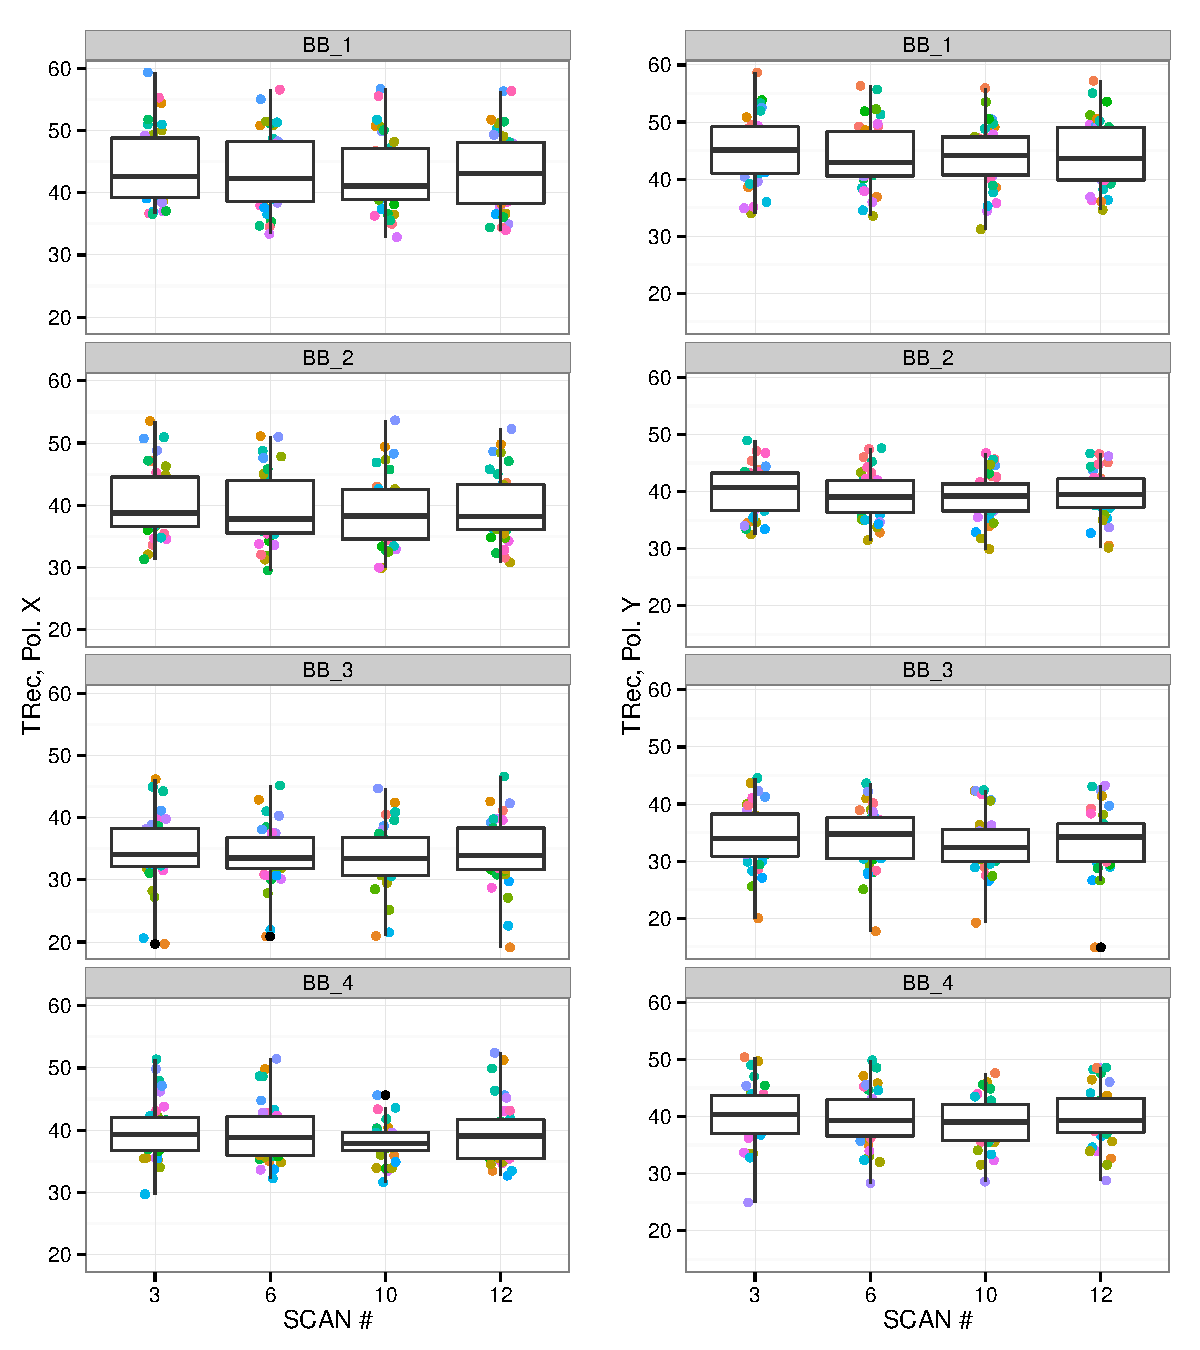
\includegraphics{QA0rep_files/figure-latex/unnamed-chunk-9-1.pdf}
\caption{}
\end{figure}

\begin{figure}[htbp]
\centering
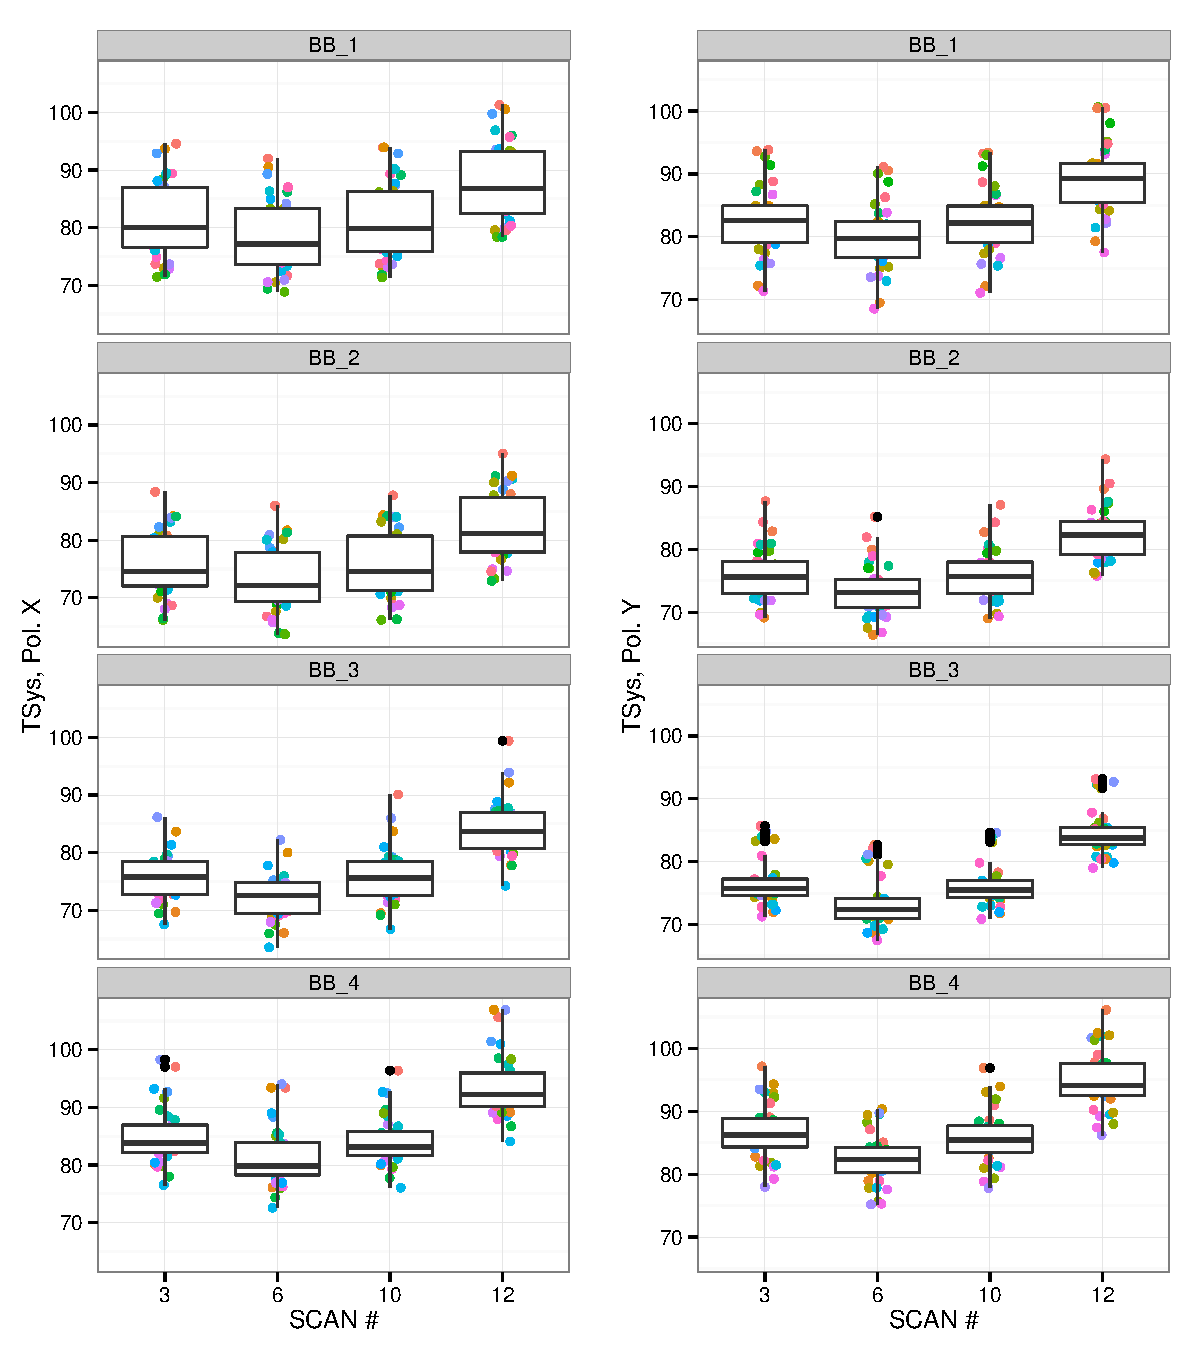
\includegraphics{QA0rep_files/figure-latex/unnamed-chunk-10-1.pdf}
\caption{}
\end{figure}

\pagebreak

\section{Phase}\label{phase}

\begin{figure}[htbp]
\centering
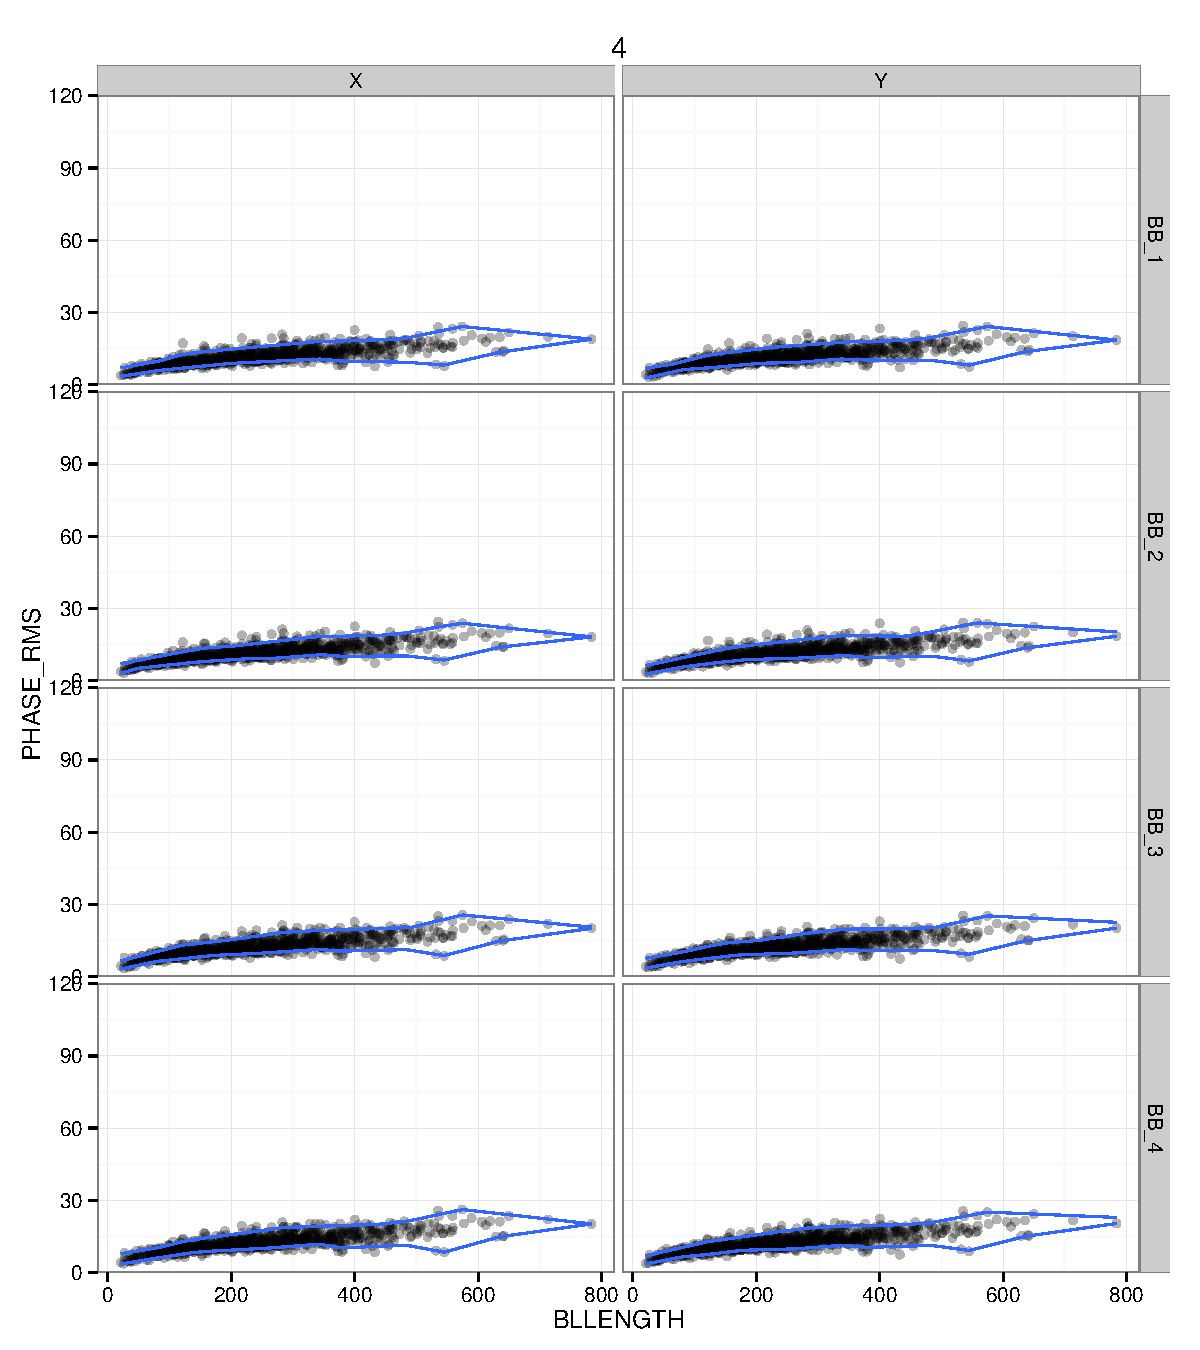
\includegraphics{QA0rep_files/figure-latex/unnamed-chunk-12-1.pdf}
\caption{}
\end{figure}

\begin{figure}[htbp]
\centering
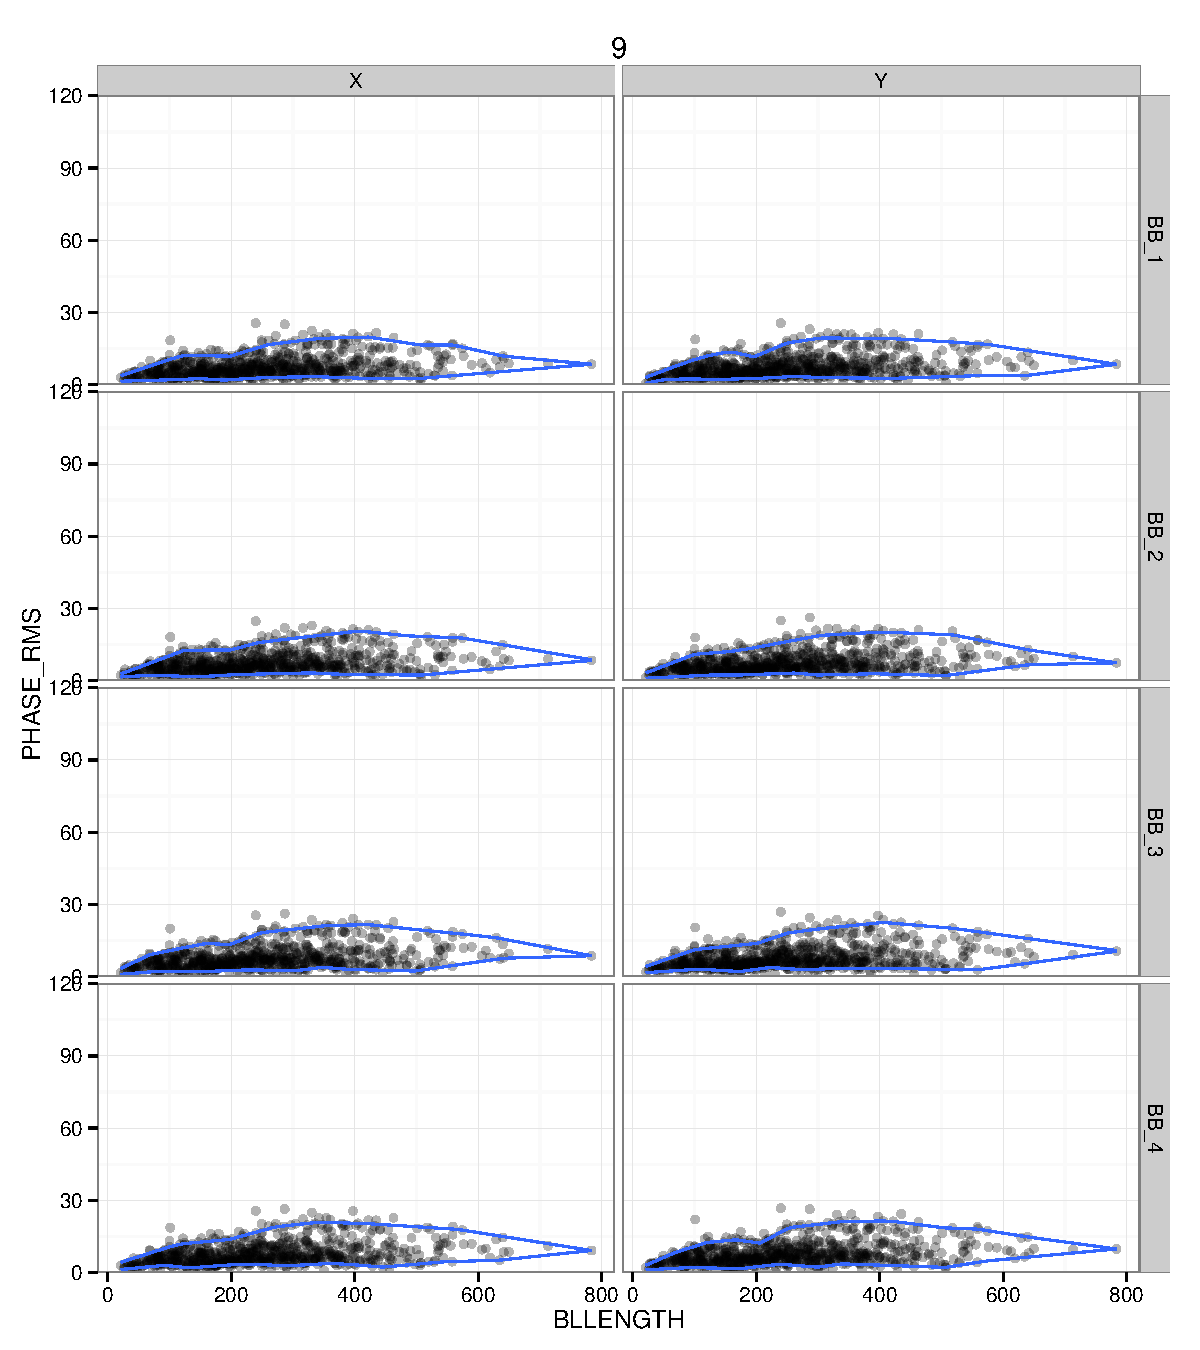
\includegraphics{QA0rep_files/figure-latex/unnamed-chunk-12-2.pdf}
\caption{}
\end{figure}

\begin{figure}[htbp]
\centering
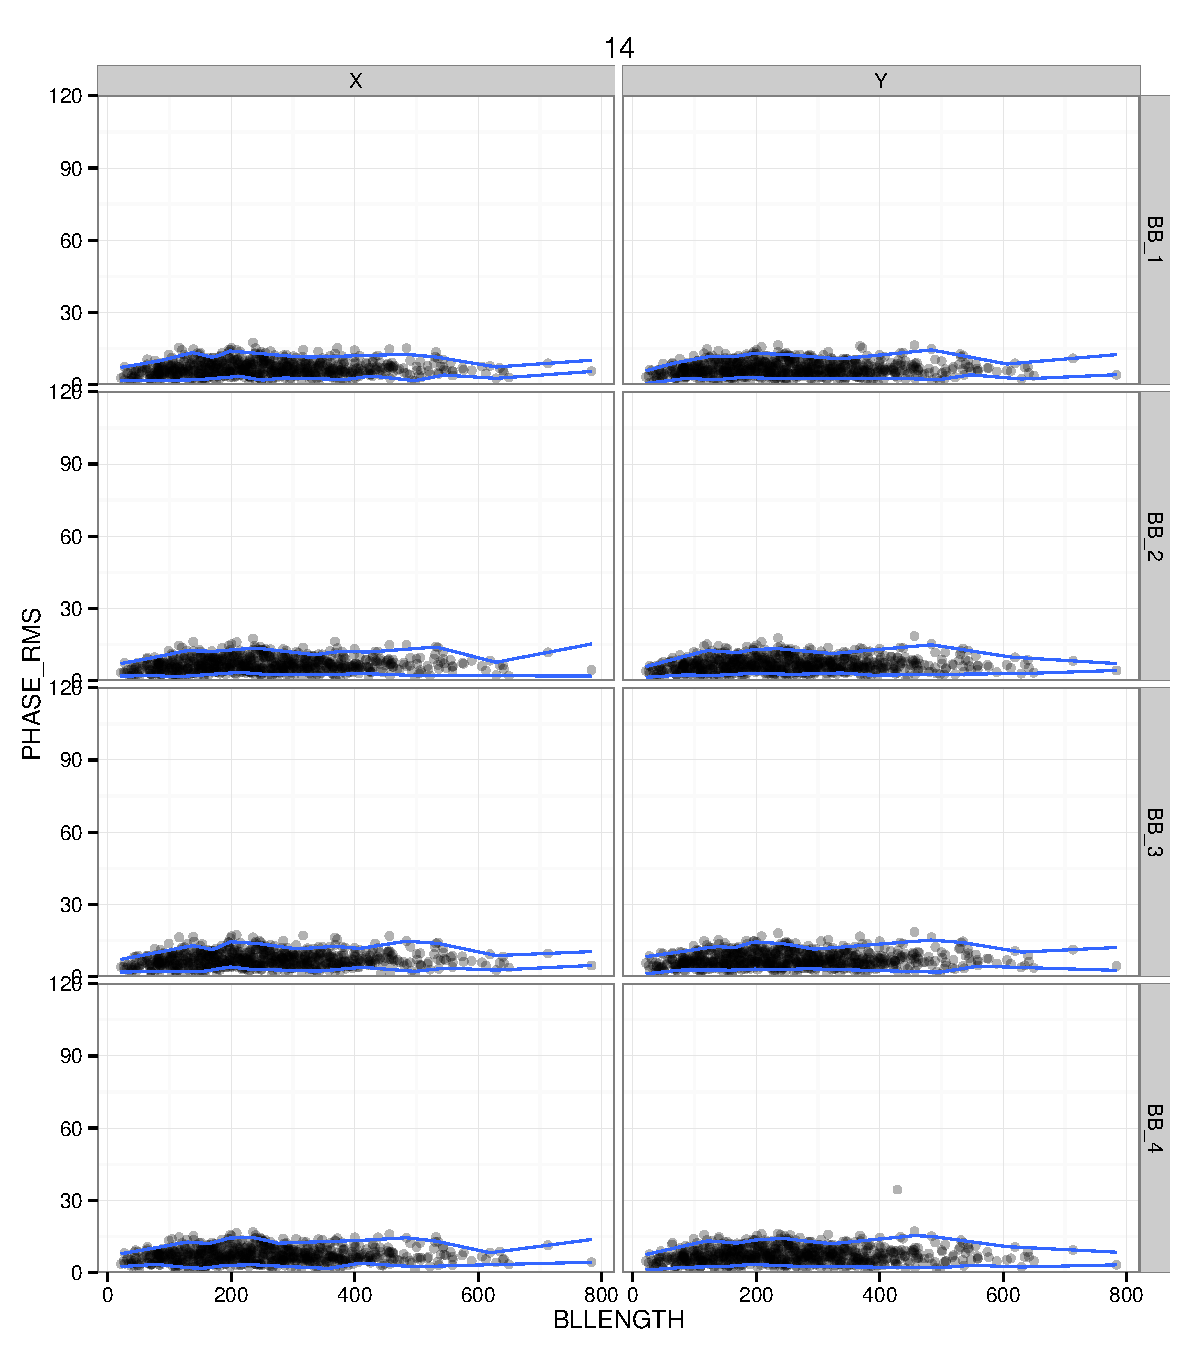
\includegraphics{QA0rep_files/figure-latex/unnamed-chunk-12-3.pdf}
\caption{}
\end{figure}

\pagebreak

\section{Delay}\label{delay}

\begin{figure}[htbp]
\centering
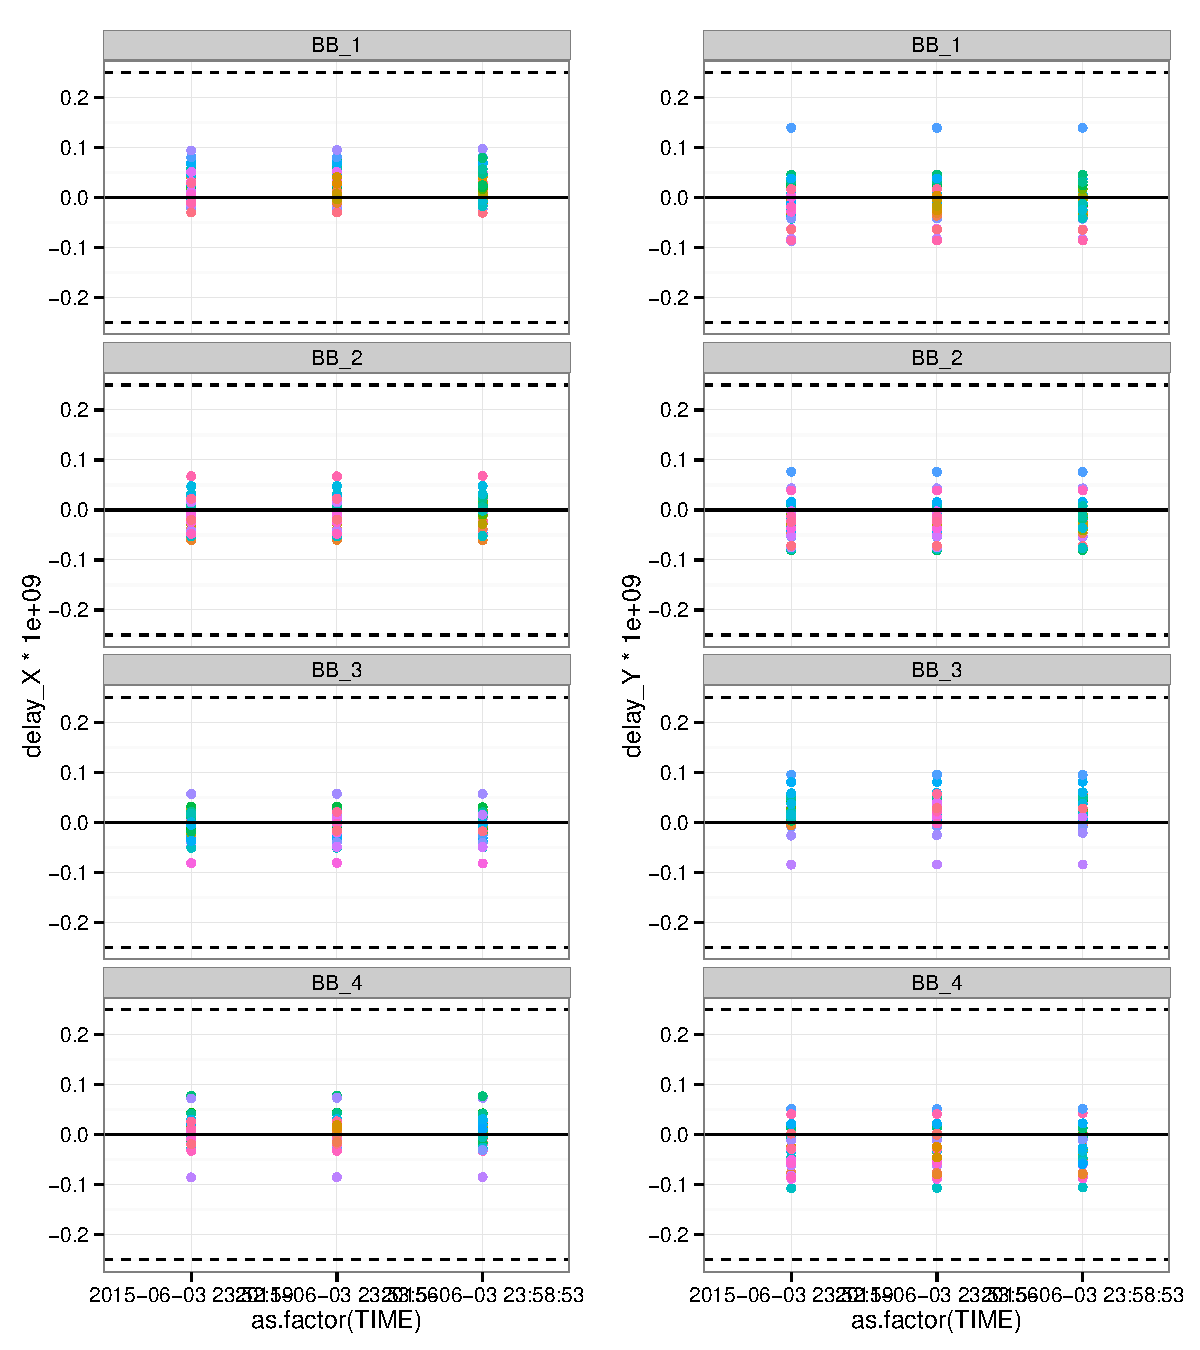
\includegraphics{QA0rep_files/figure-latex/unnamed-chunk-13-1.pdf}
\caption{}
\end{figure}

\end{document}
